\documentclass[runningheads]{llncs}
\usepackage[T1]{fontenc}
\usepackage{graphicx}
\graphicspath{{./images/}}
\usepackage{multirow}
\usepackage{longtable}
\usepackage{pdfpages}
% Used for displaying a sample figure. If possible, figure files should
% be included in EPS format.
%
% If you use the hyperref package, please uncomment the following two lines
% to display URLs in blue roman font according to Springer's eBook style:
%\usepackage{color}
%\renewcommand\UrlFont{\color{blue}\rmfamily}
%
\begin{document}
% Just after the begin
%\begin{document}
\begin{titlepage}
    \centering
    {\bfseries\LARGE International University of Ecuador \ 
    Faculty of Technical Sciences  \par}
    \vspace{1cm}
    {\scshape\Large School of Mecatronics engineering \par}
    \vspace{3cm}
    {\scshape\Huge Industrial Automatization \par}
    \vspace{3cm}
    {\itshape\Large Lab's preparatory No 3: Timer conector \par}
    \vfill
    {\Large Author: \par}
    {\Large Pablo Guacho \par Sebastian Osorio \par}
    \vfill
    {\Large Sep 20222 - Jan 2023 \par}
    \end{titlepage}
\newpage

\title{Lab's preparatory No 3 \thanks{UIDE x.}}
\author{Sebastian Osorio\inst{1}\orcidID{0000-0003-0106-5482} \and Pablo Guacho\inst{1} }

\authorrunning{P. Guacho; S. Osorio.}

\institute{International University of Ecuador, Quito Av. Jorge Fernández and Av. Simón Bolívar 170201, Ecuador
    \email{seosoriogu@uide.edu.ec}
    \url{https://www.uide.edu.ec/} }

\maketitle


\section{Timer AH3-AB }

Some of the basic charateristics of the timer AH3-AB are:
\begin{enumerate}
 \item Exclusive CMOS IC assures high performance stability, and accuracy.
 \item High repeat accuracy ± 1\%.
 \item Short resetting time-100 msec. ax.
\item Wide variety of type-14 time ranges.(0.1 sec. to 10 hrs)
\item 2 modes selectable via slide switch: Mode A(2C) for DPDT time-limiting output contacts and Mode B(1A1C) for SPDT instantaneous and time-limiting output contacts
\end{enumerate}

% Please add the following required packages to your document preamble:
% \usepackage{multirow}
% \usepackage{longtable}
% Note: It may be necessary to compile the document several times to get a multi-page table to line up properly
\begin{longtable}[c]{lc}
    \caption{Multi range timer AH3-AB specifications.}
    \label{tab:AH3-AB}\\
    \hline
    \multicolumn{2}{c}{AH3-AB Specifications}                                \\ \hline
    \endfirsthead
    %
    \multicolumn{2}{c}%
    {{\bfseries Table \thetable\ continued from previous page}} \\
    \hline
    \multicolumn{2}{c}{AH3-AB Specifications}                                \\ \hline
    \endhead
    %
    \hline
    \endfoot
    %
    \endlastfoot
    %
    \multicolumn{1}{l|}{\multirow{2}{*}{Rated   voltage}}     & AC 110V, 220V,   380V, 440V             \\
    \multicolumn{1}{l|}{}                   & DC 12V, 24V                    \\
    \multicolumn{1}{l|}{Rated   frequency}  & 50/60Hz                        \\
    \multicolumn{1}{l|}{\multirow{2}{*}{Operating   voltage}} & AC 85-110\% of rated   voltage          \\
    \multicolumn{1}{l|}{}                   & DC 80-110\% of rated   voltage \\
    \multicolumn{1}{l|}{Consumed   power}                     & 2VA for AC / About 2W   for DC          \\
    \multicolumn{1}{l|}{Control method}                       & Time-limit operation   / Self-resetting \\
    \multicolumn{1}{l|}{Contact   rating}   & 250V AC 10A (P.F.=1)           \\
    \multicolumn{1}{l|}{Ambient temp.}      & -10℃ $\sim$+55℃                \\
    \multicolumn{1}{l|}{Ambient   humidity} & 45$\sim$85\% RH                \\ \hline
    \end{longtable}

\begin{figure}[h]
    \centering
    \caption{Connection Diagram}\label{fig:ConnectionDiagram}
    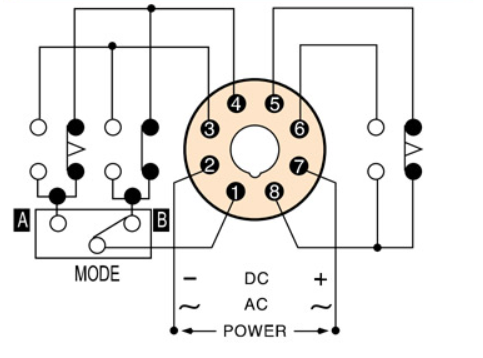
\includegraphics[scale = 0.5]{conectionDiagram.png}
\end{figure}



\begin{figure}[h]
    \centering
    \caption{Modes operation Chart}\label{fig:ModeOperation}
    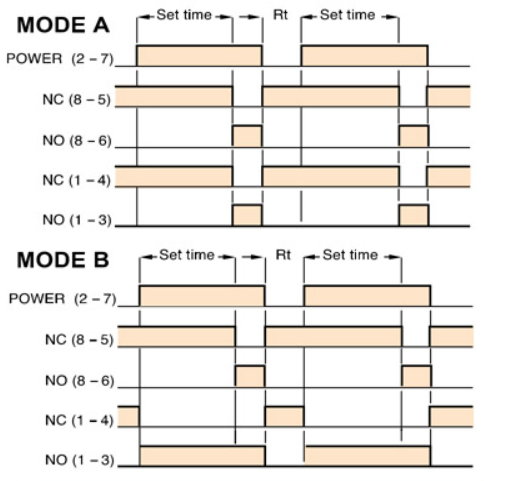
\includegraphics[scale = 0.7]{operationTime.png}
\end{figure}


\newpage

\section{Circuit proposed}
\begin{enumerate}
    \item When button S1 is pressed (momentarily), KM1 must be turned on and after a 
    time t1, contactor KM2 will turn on and KM1 will turn off. 
    \item If button S2 is pressed (momentarily), contactor KM1 and contactor KM2 will turn 
    on, and after a time t1, KM1 will turn off. 
    \item  Additionally, the circuit will have an emergency stop button S0, which will stop 
    the operation of the fans at any time. 
    \item  Include a lamp that indicates the operation of each fan. 
    \item  The design must use a timed relay (ON DELAY) and optimize the design with 
    the least number of contactor and contacts. 
    
\end{enumerate}

\newpage
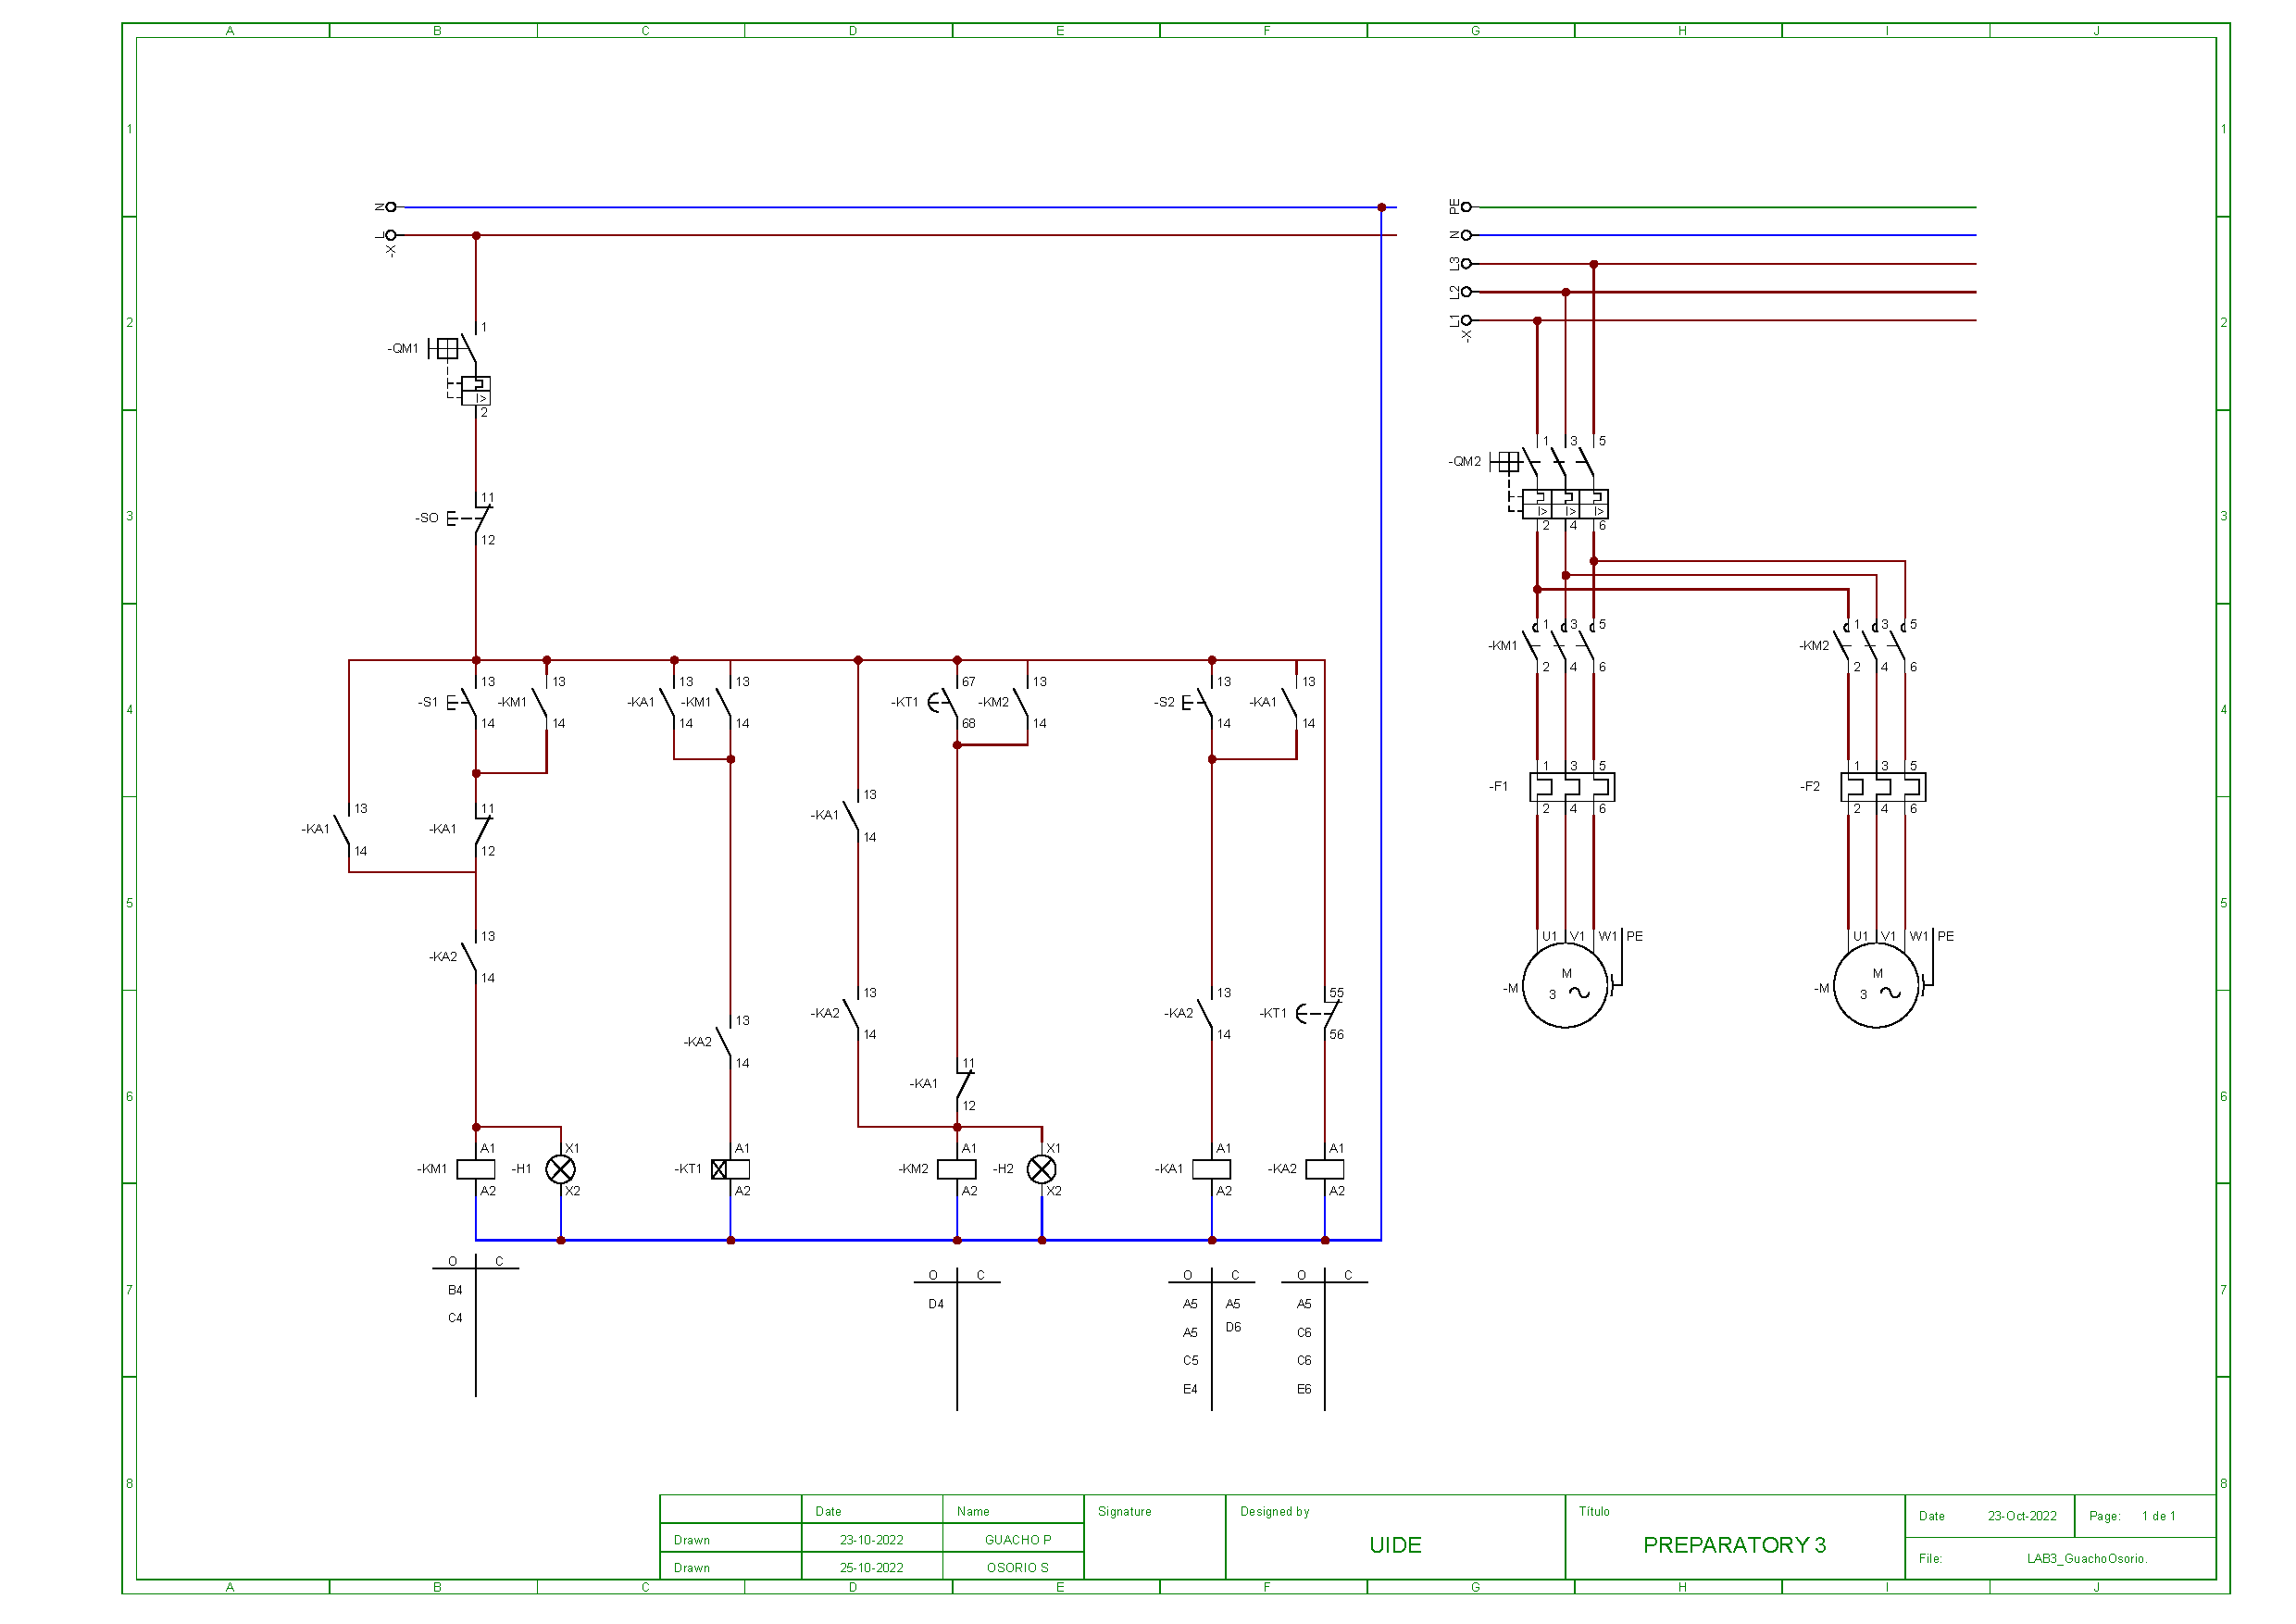
\includepdf[pages={1}]{./addons/SCHEME_A3.pdf}

% \bibliographystyle{splncs04}
% \bibliography{mybibliography}
\end{document}